\chapter{COLOMBOS: access port for cross-platform bacterial expression compendia}\label{ch:colombos}
\chaptermark{Colombos}


\instructionsintroduction

% NOTE: no abstract for each section, otherwise mess up page numbering!!
%\textbf{Abstract}
%
%\textbf{Background:} Microarrays are the main technology for large-scale 
%transcriptional gene expression profiling, but the large bodies of data 
%available in public databases are not useful due to the large heterogeneity. 
%There are several initiatives that attempt to bundle these data into 
%expression 
%compendia, but such resources for bacterial organisms are scarce and limited 
%to 
%integration of experiments from the same platform or to indirect integration 
%of 
%per experiment analysis results.
%
%\textbf{Methodology/Principal Findings:} We have constructed comprehensive 
%organism-specific cross-platform expression compendia for three bacterial 
%model 
%organisms ({\it Escherichia coli}, {\it Bacillus subtilis}, and {\it 
%Salmonella 
%enterica serovar Typhimurium}) together with an access portal, dubbed 
%COLOMBOS, 
%that not only provides easy access to the compendia, but also includes a suite 
%of tools for exploring, analysing, and visualizing the data within these 
%compendia. It is freely available at 
%\url{http://bioi.biw.kuleuven.be/colombos}. The compendia are unique in 
%directly combining expression information from different microarray platforms 
%and experiments, and we illustrate the potential benefits of this direct 
%integration with a case study: extending the known regulon of the Fur 
%transcription factor of {\it E. coli}. The compendia also incorporate 
%extensive 
%annotations for both genes and experimental conditions; these heterogeneous 
%data are functionally integrated in the COLOMBOS analysis tools to 
%interactively browse and query the compendia not only for specific genes or 
%experiments, but also metabolic pathways, transcriptional regulation 
%mechanisms, experimental conditions, biological processes, etc.
%
%\textbf{Conclusions/Significance:} We have created cross-platform expression 
%compendia for several bacterial organisms and developed a complementary access 
%port COLOMBOS, that also serves as a convenient expression analysis tool to 
%extract useful biological information. This work is relevant to a large 
%community of microbiologists by facilitating the use of publicly available 
%microarray experiments to support their research.



%\section{Introduction.new}
%Large amount of data available.
%Expression compendium, types, and their applications. (exampels)
%
%The issue with bacteria, limited amount of data, none dominant platform ...
%
%Cross-platform compendium and COLOMBOS.


\section{Introduction}

Over the last decade, the high-throughput omics technology led/driven by the 
microarray platform has revolutionized the molecular biology research. 
With the unprecedented ability to globally probe gene expressions, it was 
quickly adopted by every research lab generating colossal amount of data. 
With a few exceptions, most experiments designed to address particular 
biological question(s) are of \textit{small-scale} covering a limited set of 
experimental conditions.
Given the complexity of a living cell and its interaction with the 
environment, it has been shown that computational analysis of 
\textit{large-scale} dataset across diverse experimental conditions and cell 
types is a powerful tool to reverse engineer regulatory networks 
\cite{Faith2007, Basso2005, Ernst2008}, to study its condition dependent 
behavior \cite{Lemmens2009, Fadda2009}, and to identify compound mode of 
action  \cite{Gardner2003, Basso2005, DiBernardo2005}.
Although for many species, experiments publicly available in Gene Expression 
Omnibus (GEO) \cite{Barrett2011} or ArrayExpress \cite{Parkinson2009} cover 
a broad range of the conditions, a direct and integrated computational analysis 
of those data is not possible.
Data are segregated per experiment due to the lack of uniformity in 
reporting expression data, the heterogeneity of the microarray platforms, 
and the incomplete and inconsistent meta information specifying experimental 
conditions.

Existing compendia alleviate the aforementioned data integration issues by 
either directly integrating data across experiments albeit limited by only 
those generated on a single-platform \cite{Faith2008, Hruz2008} 
or combining results of individual experiment through meta-analysis to avoid 
direct data integration across experiments 
\cite{Rhodes2007, Pan2007, Elfilali2006, Kapushesky2010}.
Compendia created by meta-analysis are limited by the predefined  
functionalities provided by the system, hence lack of flexibility to 
incorporate new analysis.
The compendia created by direct integration, however, retain actual expression 
values, hence the compendia can be readily analysed by the existing and 
potential methods.
For eukaryotic model organisms, such a single-platform approach works well 
as the compendium based on Affymetrix chips can achieve a broad scope on 
experimental condition due to the platforms popularity.
For prokaryote, however, the single-platform constraint severely circumscribes 
the scope of the compendium created due to the lack of such a dominate platform.
For example, for model organisms such as {\it E. coli}, even the most popular 
platform `Affymetrix GeneChip E. coli Genome 2.0 Array' is used by less then 
one thirds of experiments. A significant portion of data is missed out on 
when considering only one platform.

To have the advantage of direct integration, while not being limited to a 
single platform, we have devised a strategy that directly integrates expression 
data across platforms and experiments creating a compendium provides an 
unprecedentedly broad coverage on experimental conditions.
As such a cross-platform compendium benefits most the microbiology research 
community, we have applied our method to create compendia for three 
bacteria species: \textit{Escherichia coli}, \textit{Bacillus 
subtilis}, and \textit{Salmonella enterica} serovar Typhimurium.  
Furthermore, to increase their usability for a large community of 
microbiologists, these compendia are being made available through COLOMBOS 
(COLlection Of Microarrays for Bacterial OrganismS). 
It is a web portal that provides easy access to the compendia and has an 
integrated suite of data tools for exploring, visualizing, and analysing the 
expression data.
In this Chapter, we first briefly outline the compendium methodology, then 
focus on the content of the bacterial compendia and the COLOMBOS access portal. 
Interested reader can find the detailed description about the methodology in 
Chapter \ref{ch:command}.



\section{Methods}


\subsection{Cross-platform expression compendium} 
\label{sec:colombos-comp-method}


The bacterial compendia are created following the methodology described in 
Chapter \ref{ch:command}.
It consists of three main steps designed specifically to remove the 
aforementioned hurdles that prevent direct data integration.
First, the gene expression data and the corresponding experiment and platform 
information are extracted from the experimental data directly obtained from 
GEO and ArrayExpress, removing the prevalent representation discrepancies.
%
Next, a contrast is defined between two samples, whose gene expression levels 
are measured in the same experiment, one as reference and the other as test.
The annotations are curated for each contrast by carefully analysing both the 
information stored in online database and the corresponding publication(s) when 
available, specifying both the characteristic differences (e.g. the strain 
information) and the changes in the experimental condition between the test 
and reference samples.
%
%% At last, the raw expression data are normalized using out in-house 
%% homogenization pipelines
%
At last, the raw expression data are first normalized per experiment using 
dedicated procedures that respect the characteristics of the microarray 
platform used, and subsequently log ratios are calculated for each contrast 
between its pair of carefully chosen samples, representing genes expression 
variations caused by the sample difference, the experimental condition 
difference, or the combination of two.
The log ratio calculation, capable of removing certain technical variations 
from the normalized data, inherently improves the data consistency across 
platforms and experiments \cite{Shi2006, Shi2008}.
%
Following our methodology, the compendium created is, \textit{de facto}, a 
matrix containing log-ratio expression values, in which each row correspond to 
one gene and each column one contrast.
%
\todo{COLOMBOS [pending]: providing a table for platform based data breakdown 
(cross-platform benefit)}

% original colombos section, replaced by above text due to extra chapter of 
%command

%The compendia are built in three major steps. The first step is the retrieval 
%of microarray experiments and associated platforms from Gene Expression 
%Omnibus 
%(GEO) and ArrayExpress. Representation discrepancies prevalent in experimental 
%data directly obtained from online databases are systematically removed and 
%the 
%resulting data are then stored as available in a uniform format. `As 
%available' 
%does not necessarily equate to raw scanner output, since there are no MIAME 
%reporting standards regarding the measurement units of expression 
%\cite{Brazma2001, Brazma2009}. Often raw intensities are not provided in the 
%public databases (especially for older experiments), and only already 
%processed 
%data are reported. At this stage probes are also mapped in a platform-specific 
%manner to a unique list of genes which is constructed based on the organism's 
%RefSeq file at NCBI \cite{Pruitt2007} and which corresponds to the rows of the 
%final compendium. If probe sequences are available or can be obtained from the 
%platform description, the mapping is driven by sequence homology searches 
%using 
%BLAST \cite{Altschul1997}. If not, a probe's target gene is identified by 
%other 
%probe info, namely -and in order of preference: locus tags, alternative gene 
%tags, or common gene names.
%
%In a next phase, the condition contrasts that will be represented in the 
%compendium are defined and annotated. Based on their biological role in an 
%experimental survey, hybridizations are labelled `reference' or `test' on a 
%per 
%experiment-and-platform combination basis and matched to produce a set of 
%condition contrasts. For a single channel experiment, one or more 
%hybridizations are chosen as references for the remaining tests. For dual 
%channel experiments, usually one of every two array
%hybridizations serves as a reference to the other, as this inherently counters 
%much probe spot associated variation in the measurements. There are exceptions 
%however, such as when one of the hybridizations on an array does not 
%constitute 
%an identifiable and unique biological condition for which the transcriptome 
%was 
%assessed (e.g. a sample of genomic DNA or a pool of different samples that 
%cannot be considered as biological replicates). These hybridizations are 
%discarded and the experiment is further treated as if it was a single channel 
%experiment. In this way we ensure that every contrast has a biologically 
%interpretable meaning: its associated log-ratios measure changes in expression 
%in response to quantifiable stimuli that are altered from reference to test. 
%Using a set of formal hierarchically structured condition properties 
%(representing for instance mutations, compounds in the growth medium, 
%treatments, and general growth conditions), we can then specify the annotation 
%of each condition contrast rigidly as a vector representing the differences 
%for 
%these property values between the test and reference condition. This 
%representation enables a mathematical comparison and automatic organization of 
%contrasts based on the conditions that are surveyed, but it is a labor 
%intensive manual curation process where information often needs to be 
%retrieved 
%from original publications, supplementary data and occasionally directly from 
%the authors. The condition properties themselves are further structured in a 
%condition ontology tree. This ontology employs the same classes as the Gene 
%Ontology biological process subtree terms \cite{Gene2010} and maps the 
%condition properties used to annotate the condition contrasts to one or more 
%biological processes or functionalities they most likely affect.
%
%The final part in the creation of a compendium is the homogenization of the 
%expression data: several preprocessing procedures are conducted to render 
%expression levels comparable between different experiments and platforms. 
%Crucial steps in this preprocessing are array-specific and depend on both the 
%technological platform that was used to perform the experiment, as well as on 
%the reported units of expression and the type of normalizations that might 
%have 
%already been done. In general we adhere to the following principles: 1) 
%whenever possible, raw intensities are preferred as data source over 
%normalized 
%data provided by the public repository, 2) no local background or mismatch 
%probe correction procedures are performed to avoid an increase in intensity 
%error variance for lower, less reliable intensity levels 
%\cite{Ritchie2007,Engelen2006,Li2001}, 3) non-linear normalization techniques 
%are performed to account for global inter-hybridization differences (e.g. 
%loess 
%fit to remove dye-related discrepancies on dual channel arrays 
%\cite{Yang2002}, 
%quantile normalization for high-density oligonucleotide experiments 
%\cite{Bolstad2003}) and 4) log-ratios are created for single-channel data 
%according to the condition contrast definitions and combined with the dual 
%channel measurements.


\subsection{COLOMBOS data analysis tools}
COLOMBOS provides a suite of intuitive tools for exploring, visualizing, 
and analysing the expression data in the compendia. The interface is divided in 
two main sections: a `Workspace panel' to the left and a `Data analysis panel' 
to the right (Figure \ref{fig:colombos-tools}). The workspace panel is always 
visible: it contains the main control elements and shows an overview of the 
data (the `workspace') the user is working with. The right hand data analysis 
panel is where querying of the database and visualization and analysis of the 
expression data takes place.

\begin{figure}
	\centering
  	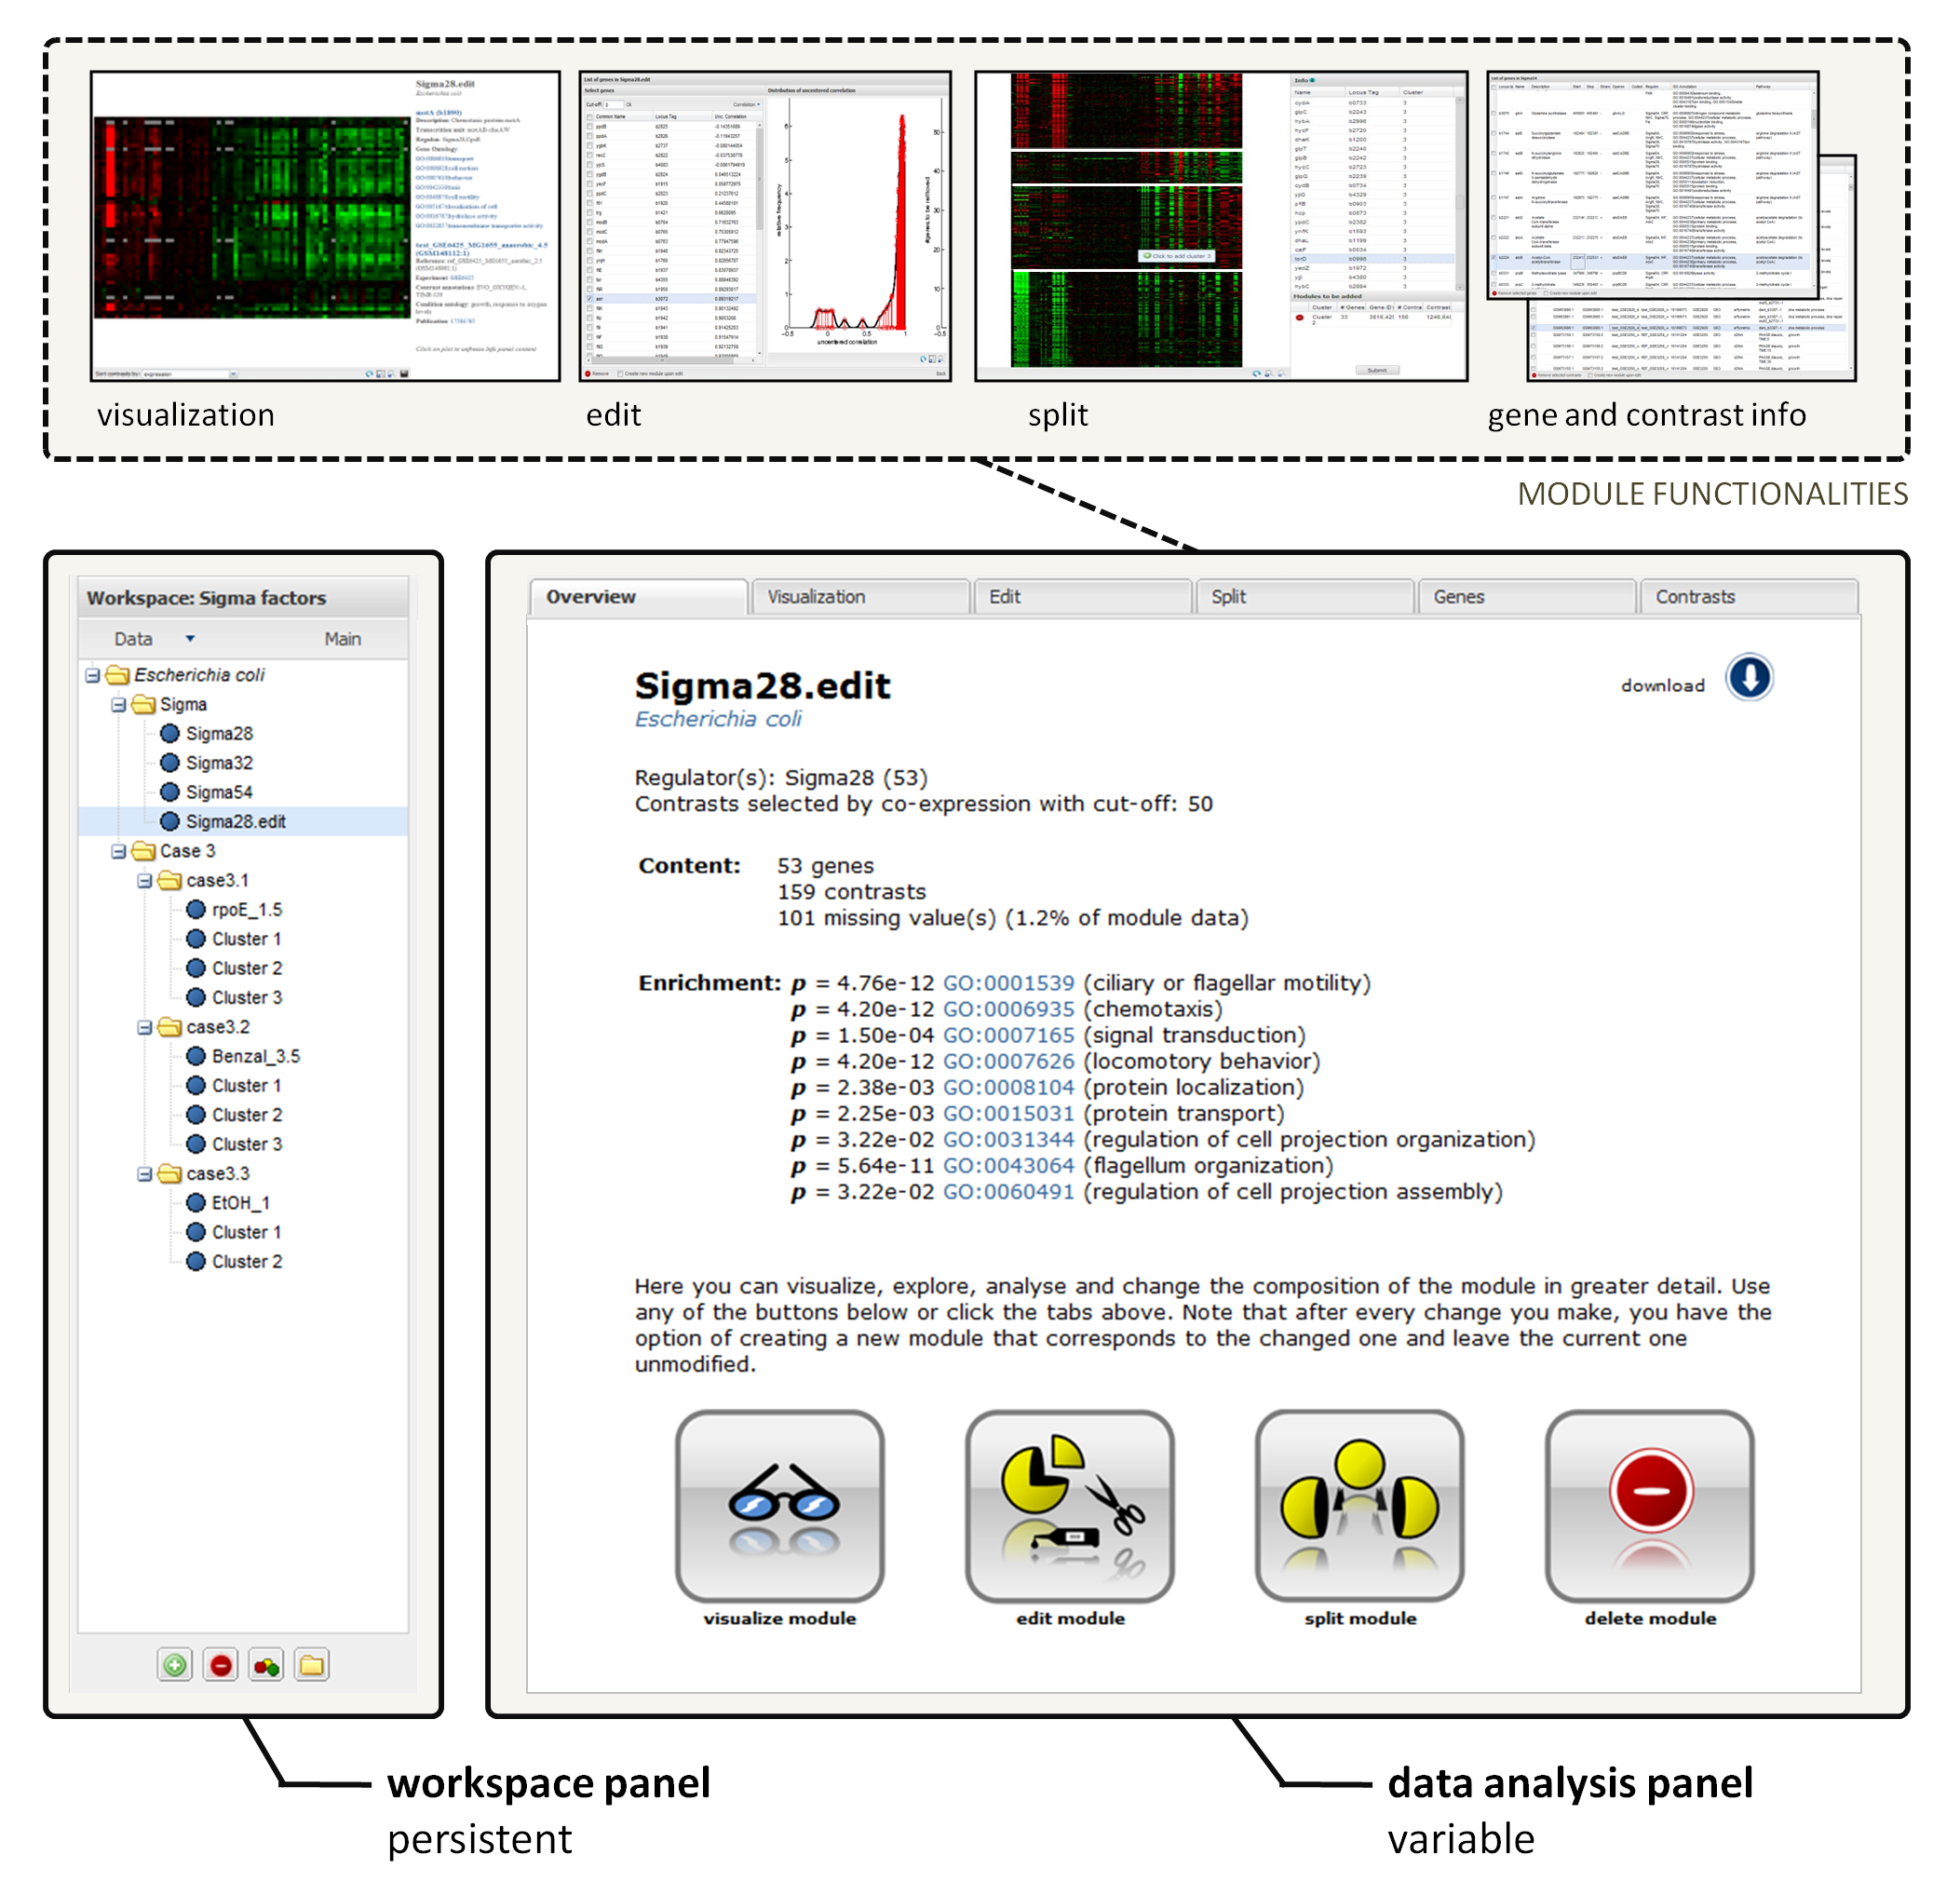
\includegraphics[width=1\textwidth]{20100813_figure1_cr.png}
  	\caption[COLOMBOS data analysis components]{\textbf{COLOMBOS data analysis 
  	components}. 
  	The bottom part shows the two main panels of the data analysis 
  	page. The left hand workspace panel is always visible, containing an 
  	overview of the modules and the main analysis controls. The content of the 
  	right hand data analysis panel depends on the actions of the user. In this 
  	case it shows the overview page for a module selected in the workspace. 
  	This overview page not only provides some general information on the 
  	selected module, but also serves as a guide for further examination and 
  	analysis steps. These are illustrated at the top part of the figure and 
  	include visualization, content editing (demonstrated is the removal of 
  	genes based on expression profile similarity), splitting the module based 
  	on expression values (shown here in the gene direction), and exploration of 
  	gene and contrast information.}
  	\label{fig:colombos-tools}
\end{figure}


All steps and procedures in the COLOMBOS analysis tools act on what we call 
expression `modules'. A module in COLOMBOS can be considered as a result of a 
single query to the database and is always a combination of a set of genes and 
a set of contrasts with corresponding expression values. Modules are dynamic in 
that at any time after creation their content can be altered by the user in 
various ways. In addition, multiple modules can be retained and organized in 
the workspace and can be analysed simultaneously. As the basic modus operandi, 
modules create a general framework through which various interesting, but 
conceptually different biological questions can be handled.

Three different options are given for creating a module: by manually selecting 
only genes and have COLOMBOS automatically identify relevant condition 
contrasts, by manually selecting only condition contrasts and have COLOMBOS 
automatically identify sets of co-expressed genes, or by explicitly selecting 
both genes and condition contrasts manually. Depending on the gene annotations 
that are available for the selected organism in the public databases that 
COLOMBOS integrates (see Table \ref{tab:colTB-overview}), the set of genes can 
be selected as anything from an operon or a regulon, to enzymes representing a 
metabolic pathway, or any custom list of genes that one is interested in. 
Similarly, the module contrasts represent the biological conditions of interest 
and can also be retrieved in various ways, such as by experiment, by contrast 
annotation, or by condition ontology. When specifying only a set of genes, 
COLOMBOS will identify relevant condition contrasts based on the expression 
values of the selected genes in the compendium (user defined relevance cut-off 
that prioritizes both the magnitude as well as the consistency of the 
expression changes; see Appendix \ref{ch:apd-colombos} for more details). 
Starting from only condition contrasts, COLOMBOS retrieves the most variable 
genes for the defined contrasts and (as an optional step) can identify clusters 
of co-expressed genes within this selection, which can be added as distinct 
modules.

Once a module is defined, it can be visualized in an interactive manner (with 
the option to export high-quality images), its expression values and contrast 
annotation can be downloaded, it can be split up in multiple modules in either 
the gene or contrast direction by clustering the expression profiles, or it can 
be further edited in gene and/or contrast composition by using available gene 
and contrast annotations or by analysis of the expression values in the 
compendium. These functionalities of the analysis tools are illustrated in 
Figure \ref{fig:colombos-tools}, showing the overview page for a single module. 
The module overview page gives some basic module information (such as the 
number of included genes and contrasts, the number of missing values, and a 
list of Gene Ontology enrichment scores) and serves as a helping guide to 
further analyse and visualize the module's composition.

When multiple modules have been created, they can also be explored and edited 
together. Any number of modules can be collectively visualized (to explore 
potential overlap), can be merged into a new module, and can be subtracted from 
one another in gene or contrast content. Visually exploring the module overlap, 
both in gene and contrast composition, can serve as an important guide for 
deciding which modules may be grouped or subtracted.

Note that all of COLOMBOS' calculations, in both creating and editing modules, 
explicitly take into account the relative nature of the expression values by 
recognizing $0$, implying no change, as the natural reference state of a 
log-ratio (details in Appendix \ref{ch:apd-colombos}). 
Gene profile similarities are calculated by default as the uncentered Pearson 
correlation, which assumes that the sample means (i.e. the means of two gene 
expression profiles across a set of condition contrasts) are zero. Standard 
deviations of gene profiles are calculated in a similar way (as the root of the 
mean sum of squared log-ratios)



\section{Results}

\subsection{Becteria compendia}\label{sec:colombos-comp}

Currently COLOMBOS provides access to fully annotated public expression 
compendia for three bacterial model organisms: {\it Escherichia coli}, {\it 
Bacillus subtilis}, and {\it Salmonella enterica} serovar Typhimurium (see 
Table \ref{tab:colTB-overview} for an overview of their respective 
content). 
These expression compendia are essentially organism-specific matrices of 
expression values derived from publicly available microarray experiments which 
are homogenized to make them comparable. The rows of a compendium matrix 
correspond to the known genes of the organism in question. Each column is a 
`condition contrast' because it does not represent single experimental 
condition, but in fact always represent the difference between a 
test and reference condition (the expression values themselves are calculated 
as expression log-ratios). 
%
Converting absolute measures of expression into 
expression changes is the principal means for rendering expression values 
comparable across platforms and experiments. Relative expression calculated 
intra-experiment/platform (i.e. between two conditions measured in the same 
microarray experiment using one platform) negates much of the platform and 
experiment specific variations that makes it impossible to reliably compare the 
absolute quantities reported in different experiments \cite{Shi2006}.
\todo{COLOMBOS [pending]: Update the data to version 2}

\begin{table}
	\caption{An overview of the content of the three bacteria expression 
	compendia}
	\label{tab:colTB-overview}
	\begin{small}
	\begin{tabular}{@{}l c c c@{}}
	\toprule
	& & & {\bf\it\small Salmonella} \\
	& {\bf\it\small Escherichia} & {\bf\it\small Bacillus} & {\bf\it\small enterica serovar} \\
	& {\bf\it\small coli} & {\bf\it\small subtilis} & {\bf\it\small  Typhimurium} \\
	\midrule
	{\bf Number of genes} 		& 4295 & 4105 & 4525 \\
	{\bf Number of contrasts} 	& 1429 & 259 & 717 \\
	{\it ~~~source DB} 			& GEO, AE & GEO & GEO \\
	{\it ~~~microarrays} 		& 1483 & 265 & 723 \\
	{\it ~~~experiments}	 	& 84 & 9 & 25 \\
	{\it ~~~platforms} 			& 35 & 13 & 9 \\
	{\bf Missing values} 		& 6.1\% & 6.40\% & 3.90\% \\
	{\bf Condition properties} 	& 242 & 67 & 77 \\
	{\bf Condition ontology terms} & 56 & 24 & 23 \\
	\multicolumn{4}{l}{\bf External DBs} \\
	{\it ~~~pathway} 			& EcoCyc & BioCyc & BioCyc \\
	{\it ~~~regulon} 			& RegulonDB & DBTBS & \\
	{\it ~~~operon} 			& EcoCyc & BioCyc & BioCyc \\
	{\it ~~~GO} 				& UniProt GOA & UniProt GOA & UniProt GOA \\
	\bottomrule
	\end{tabular}
	\end{small}
\end{table}



In order to be able to interpret and compare the expression log-ratios across an entire compendium, we have extensively annotated all contrasts using a set of formal hierarchically-structured condition properties (representing for instance mutations, compounds in the growth medium, treatments, and general growth conditions). This contrast annotation is done to structure the large amounts of potentially useful information that remain untapped due to the non-standardized condition descriptions in public databases. The annotation is complemented with a condition ontology that groups the condition properties under one or more ontology terms. It serves as a higher level organization, and provides a biologically more intuitive view of the condition contrast annotation by assigning properties of seemingly distinct categories to the same biological process. For example, in our {\it Escherichia coli} compendium the condition ontology term `response to oxygen levels' includes condition properties that are linked to cellular processes that are dependent on oxygen availability, such as {\it fnr} mutations (a global oxygen responsive transcriptional regulator), NO$_2$ concentration (an electron transport decoupler), agitation of the growth medium, actual oxygen levels, etc. Apart from a thorough description of the represented biological conditions, we have incorporated several sources of information from main curated databases (UniProt GOA \cite{Camon2004}, EcoCyc \cite{Keseler2009}, BioCyc \cite{Caspi2008}, RegulonDB \cite{Gama-Castro2008}, and DBTBS \cite{Sierro2008}) into each of the microbial compendia. This includes additional data regarding gene function and genomic organization, metabolic pathways, and transcriptional regulation mechanisms. Both the condition annotation and additional gene information are integrated into the COLOMBOS data analysis tools in a functional manner to interactively browse and query the compendia (see Methods). If users so desire however, they can download the compendia in their entirety.


\subsection{Case study - Fur regulatory targets}
In the following case study we illustrate the benefits of exploiting the direct 
integration of expression values, as well as the ease with which one can make 
interesting biological discoveries using the COLOMBOS data analysis tools (see 
Methods for a detailed description of their functionalities). A straightforward 
application provided by COLOMBOS is the ability to find genes which show 
similar expression behavior with a starting set of genes for relevant condition 
contrasts. Since co-expression might infer co-regulation, we can use this 
approach to obtain a list of potential target genes that might also be 
regulated by the same transcription factor. In this example, we will use 
COLOMBOS to identify novel potential targets for the Fur transcription factor 
of {\it Escherichia coli}. Fur mostly regulates genes related to iron 
homeostasis and is strongly conserved across many Gram-negative and 
Gram-positive bacteria \cite{Chen2007}. It has received a lot of interest in 
the past for its role in iron-limited conditions, such as those encountered by 
pathogenic strains in their hosts \cite{Panina2001}. Fur has mostly been 
reported as a direct repressor of its target genes, but is considered a dual 
regulator: activation occurs indirectly by transcriptional repression of a 
small antisense RNA RhyB \cite{Masse2002}. Fur has also been known to mediate 
combinatorial responses along with many other transcription factors 
\cite{Patzer2001, Zhang2005}. In the latest release of RegulonDB 
\cite{Gama-Castro2008}, Fur is described as having 98 target sites in 43 
distinct promoters, with 28 of these promoters known to be subject to 
combinatorial regulation. The results of all data analysis steps discussed here 
are available in the case study data set accessible from the COLOMBOS home page.

An initial set of 39 genes of the Fur regulon was constructed using the 
regulatory information integrated in COLOMBOS. Only genes known to be regulated 
by Fur alone, or by Fur in combination with the global regulators CRP, H-NS 
and/or FNR were selected. All other cases where known combinatorial regulation 
could occur were not included in the initial set because they might result in 
more complex, less homogeneous transcriptional responses. For similar 
considerations, if the activating sigma factor was known, only genes responsive 
to the household s70 were retained in the initial set. For this initial gene 
set the most relevant condition contrasts in the compendium were then selected, 
i.e. the contrasts where these genes showed the highest and most coherent 
response: a relevance cut-off (see Supplementary Text S1) of 1 resulted in 97 
contrasts. Not all of the retained genes show a similar expression profile for 
the retained contrasts however, which might be attributed to unknown active 
forms of combinatorial regulation or the dual regulatory function of Fur. Since 
we wanted to continue with a set of strongly co-expressed genes, COLOMBOS was 
used to further clean the initial gene set by removing genes that had a 
correlation smaller then 0.8 with the mean of the initial set for the selected 
contrasts. Next we used COLOMBOS to extend the remaining set of 30 genes with 
additional ones that follow the same expression pattern for the selected 
contrasts (a correlation bigger than 0.8 was used as cut-off value), under the 
assumption that these constitute potential Fur targets. In this way, 19 extra 
genes were retrieved (Table \ref{tab:colTB-case}), 7 of which were part of the 
Fur regulon but were not included in the initial set because they were known to 
be subject to regulation by additional transcription factors. The fact that 
these Fur-regulated genes were nevertheless retrieved might indicate that the 
additional combinatorial regulation was not active under the surveyed 
conditions.


\todo{COLOMBOS: make sure it is at odd page}
%
\begin{sidewaystable}
\centering
\caption{Finding potential novel Fur targets – a case study}
\label{tab:colTB-case}
\begin{scriptsize}
% NOTE: to redefine the alignments of column in tabular env. requires load package 'array'!
\begin{tabular}{ l c >{\raggedright}p{4cm} c c c 
>{\centering\arraybackslash}p{1.2cm} >{\raggedright\arraybackslash}p{4cm} }
	\toprule
	\textbf{{\scriptsize Locus tag}} & \textbf{{\scriptsize Name}} & 
	\textbf{{\scriptsize Description}} & \textbf{{\scriptsize Operon}} & 
	\textbf{{\scriptsize Known}} & \textbf{{\scriptsize COLOMBOS}} & 
	\textbf{{\scriptsize Meta analysis}} & \textbf{{\scriptsize Evidence}} \\
	\midrule
	
	b1681 & \textit{sufD} & SufBCD Fe-S cluster scaffold & \textit{sufABCDSE} & 
	+ &		& + & Fur, OxyR, IHF, lscR \\[1ex]
	
	b1683 & \textit{sufB} & SufBCD Fe-S cluster scaffold & \textit{sufABCDSE} & 
	+ & + 	& 	& Fur, OxyR, IHF, lscR \\[1ex]
	
	b2392 & \textit{mntH} & Manganese transport protein & \textit{mntH} & 
	+ & + 	& + & Fur, MntR \\[1ex]
	
	b2673 & \textit{nrdH} & Glutaredoxin-like protein 	& \textit{nrdHIEF} &
	+ & + 	& + & Fur, NrdR \\[1ex]
	
	b2674 & \textit{nrdI} & Not annotated 				& \textit{nrdHIEF} & 
	+ & + 	& + & Fur, NrdR \\[1ex]
	
	b2675 & \textit{nrdE} & Ribonucleoside-P$_i$ reductase 2 $\alpha$ & 
	\textit{nrdHIEF} & 
	+ & + 	& + & Fur, NrdR \\[1ex]
	
	b2676 & \textit{nrdF} & Ribonucleoside-P$_i$ reductase 2 $\beta$ & 
	\textit{nrdHIEF} & 
	+ & + 	& + & Fur, NrdR \\[1ex]
	
	b4291 & \textit{fecA} & Fe3+ dicitrate transport protein & 
	\textit{fecABCDE} & 
	+ & + 	& 	& Fur, CRP, PdhR \\[1ex]
	
	b0468 & \textit{ybaN} & Inner membrane protein 		& \textit{ybaN} & 
	  & + 	& 	& Predicted \\[1ex]
	  
	b0804 & \textit{ybiX} & PKHD-type hydroxylase 		& \textit{ybiX} & 
	  & + 	& 	& Predicted; Fur dependent expression \\[1ex]
	  
	b1018 & \textit{efeO} & UPF0409 protein 		& \textit{efeUOB} & 
	  & + 	& 	& Predicted; functional in related strain \\[1ex]
	  
	b1452 & \textit{yncE} & Uncharacterized protein & \textit{yncE} & 
	  & + 	& + & Fur dependent expression \\[1ex]
	  
	b1494 & \textit{pqqL} & Probable zinc protease 	& \textit{pqqL} & 
	  & + 	& 	& Potential operon \textit{yddAB\_pqqL} \\[1ex]
	  
	b1495 & \textit{yddB} & Uncharacterized protein & \textit{yddAB} & 
	  & + 	&	& Predicted \\[1ex]
	  
	b1705 & \textit{ydiE} & Not annotated 			& \textit{ydiE} & 
	  & + 	& 	& Predicted; Fur dependent expression \\[1ex]
	  
	b2211 & \textit{yojI} & ATP-binding ABC transporter & \textit{yojI} & 
	  & + 	& 	& \\[1ex]
	  
	b3070 & \textit{yqjH} & Uncharacterized protein & \textit{yqjH} & 
	  & + 	& + & Predicted \\[1ex]
	  
	b3337 & \textit{bfd} & Bacterioferritin-associated ferredoxin & 
	\textit{bfd-bfr} & 
	  & + 	& 	& Indirect RhyB regulatio \\[1ex]
	  
	b3410 & \textit{feoC} & Ferrous iron transport protein C & \textit{feoABC} 
	& 
	  & + 	& 	& TU \textit{feoABC} with \textit{feoA} known target \\[1ex]
	  
	b4366 & \textit{bglJ} & Transcriptional activator protein & 
	\textit{yjjQ-bglJ} & 
	  & + 	& 	& \\[1ex]
	\bottomrule
\end{tabular}
\end{scriptsize}
\end{sidewaystable}





Of the 12 novel genes, most showed a high likelihood of being Fur targets 
(Table \ref{tab:colTB-case}). Six of these genes (\textit{yqjH}, \textit{ydiE}, 
\textit{ybaN}, \textit{yncE}, \textit{yddB} and \textit{ybiX}) were previously 
predicted to have a Fur target site in their transcription unit promoter by at 
least one of two independent studies \cite{Panina2001, Meysman2011} (in case of 
\textit{ybiX} as part of the proposed \textit{fiu}\textunderscore\textit{ybiX} 
operon). Transcription of three of these (\textit{ydiE}, \textit{yncE} and 
\textit{ybiX}) was moreover shown to be altered in a specific 
Fe$^{2+}$-Fur-dependent manner \cite{McHugh2003} and while little is known with 
regard to their function, the \textit{ybiX} gene encodes a protein similar to 
an iron-regulated hydroxylase-encoding gene from {\it Pseudomonas aeruginosa}, 
further supporting a role for Fur in its transcriptional regulation. 
\textit{pqqL} presents an interesting case: it encodes for a putative zinc 
peptidase and is situated directly downstream of the predicted 
Fur regulated \textit{yddAB} operon in the chromosome. 
%
Using COLOMBOS to select the most relevant 
condition contrasts for the three genes \textit{yddA}, \textit{yddB}, and 
\textit{pqqL} (see loadable case study data set) indeed shows that these genes 
are subject to tight co-expression, opening up the possibility of them being 
transcribed as a single transcription unit and putting \textit{pqqL} under 
influence of the \textit{yddA} promoter. The \textit{feoC} gene is annotated as 
part of \textit{feoABC} transcription unit as of the latest RegulonDB release 
(v6.8), which was not yet incorporated in COLOMBOS at the time of the analysis. 
This places it under the influence of the \textit{feoA} promoter, which is a 
known Fur target. The \textit{bfd} gene is clearly functionally related to Fur, 
being involved in iron storage and release, and has predicted binding sites in 
its promoter \cite{Chen2007}. \textit{bfd} is also the first gene in the 
\textit{bfd}\textunderscore\textit{bfr} operon, \textit{bfr} encoding for an 
iron storage protein that is at the very least indirectly regulated by Fur as 
it has been shown that the expression of this gene is repressed by a small RNA 
RhyB, which in turn is repressed by Fur \cite{Masse2002}. The complex Fur 
dependent regulation of \textit{bfd}\textunderscore\textit{bfr} is also 
apparent by diverging expression responses for some of the selected contrasts. 
In the {\it E. coli} K12 strain, the gene \textit{efeO} is part of an operon 
that has been disrupted due to a frame shift mutation. However, a Fur binding 
site was recently predicted in the \textit{efeU} promoter \cite{Meysman2011} 
and it has been shown in the related {\it E. coli} Nissle 1917 strain that 
expression of \textit{efeUOB} increases in response to iron-depleted conditions 
in a Fe$^{2+}$-Fur-dependent manner \cite{Grosse2006}.

COLOMBOS also provides the functionality to retrieve anti-correlated genes, 
which can be interesting to investigate the potential of dual regulation 
(activation or repression by the same regulator). In the case of our Fur 
module, none of the anti-correlated genes pass the threshold of 20.8, but it is 
interesting to note that the second best ranked gene (correlation 20.74) is 
{\it ftnA}. This gene was not yet assigned as a Fur target in the RegulonDB 
release included in COLOMBOS, but it was recently shown that {\it ftnA} is 
transcriptionally activated by Fur directly (as opposed to indirectly through 
RhyB as is usually the case for Fur mediated activation) by reversal of H-NS 
silencing \cite{Nandal2010}.

While the retrieval of already known Fur regulon genes combined with a set of likely targets confirms that a careful co-expression analysis can lead to the identification of novel targets, this does not imply that the direct integration of expression data itself, as in our compendia, provides any benefits. To illustrate the advantage of using cross-platform compendia, we repeated the analysis on a per experiment basis (a `meta-analysis' of 7 experiments from which the 97 contrasts above were selected). Note that, to maximize the quality of the results of this meta-analysis, we did not use all contrasts within each experiment, but only the most relevant ones (selected with the same relevance cut-off as before), and that we ignored experiments with two contrasts or less. When extending the initial 30 genes with the same correlation cut-off of 0.8, the number of additional genes for each experiment ranges between 389 and 1385, the union adding up to a total of 3361. Most of these genes are false-positives with respect to being members of the Fur regulon: within single experiments generally only a limited number of similar conditions are surveyed and this increases the chance of finding genes with similar up and down regulation patterns but not sharing the exact same regulatory program. Trying to counter this effect by increasing the correlation cut-off does not necessarily yield better results, a cut-off of 0.9 resulting in the union containing 2135 additional genes, one of 0.95 in 1361 genes. Therefore we retained only the intersection, i.e. those genes that were added by each of the per experiment extensions with a correlation cut-off of 0.8. This intersection constituted 8 additional genes (a cut-off of 0.9 resulted in only 4 added genes, 0.95 resulted in none), 6 of them already known Fur targets, and only two uncharacterized genes representing potential novel targets. All of these were also retrieved by the COLOMBOS cross-platform analysis, with the exception of a single already known Fur target, {\it sufD}. However, another gene of the {\it sufABCDSE} operon was selected by the cross-platform analysis ({\it sufB}; all other genes of the operon showed correlations with the initial set of just under 0.8), retrieving the same promoter as a Fur target.



\section{Conclusions and future directions}

%\todo{[colombos]Move future directions into the last chapter}

\begin{sidewaystable}
	\centering
	\begin{threeparttable}
	\begin{small}
	\caption{Conceptual comparison of COLOMBOS with similar initiatives}
	\label{tab:colTB-comp}
%	\begin{tabular}{p{3cm} p{4cm} p{4cm} p{4cm} p{5cm}}
%	\begin{tabular}{p{2cm} p{2.2cm} p{2cm} p{2cm} p{2.3cm}}
	\begin{tabular}{ >{\raggedright}p{0.13\linewidth} 
	>{\raggedright}p{0.2\linewidth} >{\raggedright}p{0.15\linewidth} 
	>{\raggedright}p{0.22\linewidth} >{\raggedright}p{0.18\linewidth} @{}}
	
		\toprule
		 & {\centering\bf\small COLOMBOS} & {\centering\bf\small M3D} & 
		 {\centering\bf\small GXA} & {\centering\bf\small GeneVestigator} 
		 \tabularnewline
		\midrule
		\multicolumn{5}{l}{\bf Database Content} \tabularnewline
		\hline
		Expression data\tnote{1} & Cross-platform compendia & Single platform 
		compendia (Affymetrix) & Experiment centered (ArrayExpress 
		meta-analysis) & Single platform compendia 
		(Affymetrix)\tabularnewline[1ex]
		\arrayrulecolor{Gray}\hline
		Organisms & Prokaryotes (3) & Prokaryotes (2) and a eukaryote & 
		Eukaryotes (10) & Eukaryotes (9) and a prokaryote \tabularnewline[1ex] 
		\arrayrulecolor{Gray}\hline
		Gene annotation & Incroporation of multiple species-specific DBs & 
		Referal to SGD, BioCyc & EBI & None\tabularnewline[1ex] 
		\arrayrulecolor{Gray}\hline
		Microarray annotation & Microarray annotation and condition 
		ontology\tnote{2} & Microarray annotation & Microarray annotation and 
		condition ontology\tnote{2} & Microarray annotation 
		\tabularnewline[1ex] 
		\arrayrulecolor{Gray}\hline
		Tools suite & Interactive visualization, expression analysis & 
		Visualization, expression analysis & Interactive visualization, 
		expression analysis & Interactive visualization, expression analysis 
		\tabularnewline
		\arrayrulecolor{Gray}\hline
		
		\arrayrulecolor{Black}
		%\tabularnewline[-2.5ex] % add a bit of space, break right vertical line
		\multicolumn{5}{l}{\bf Functionalities}
		\tabularnewline
		\hline
		Expression analysis\tnote{3} & Multiple queries & Single query & Single 
		query & Single query (limited) \tabularnewline[1ex] 
		\arrayrulecolor{Gray}\hline
		Query genes by \ldots & Gene IDs; functional or structural 
		characteristics & Gene IDs & Gene/protein IDs & Gene IDs 
		\tabularnewline[1ex] 
		\arrayrulecolor{Gray}\hline	
		Query arrays by \ldots & Experiment, annotation, or ontology & 
		Experiment, annotation & Experiment, annotation, or ontology & 
		Annotation \tabularnewline[1ex] 
		\arrayrulecolor{Gray}\hline
		Download & Analysis results and/or entire compendia & Analysis results 
		and/or entire compendia & Only experiments indirectly (through 
		ArrayExpress) & Analysis results (limited) \tabularnewline
		\arrayrulecolor{Black}\bottomrule 
	\end{tabular}
	\end{small}
	\begin{tiny}
	\begin{tablenotes}
		\item[1] Compendium: a data matrix (genes in rows, microarrays in 
		columns) combining expression measurements from different experiments 
		(an experiment being a set of microarrays submitted to the public DBs 
		as such, implying that they were performed by the same lab and on the 
		same technological platform). Single- vs. cross-platform: combining 
		data from the same technological platform is relatively easy as the 
		same preprocessing methodology can be employed; COLOMBOS is unique in 
		combining data from different platforms using a specialized 
		homogenization pipeline. Meta-analysis: expression data are not 
		combined directly but experiments are analysed separately where after 
		the results are compared.
		\item[2] The biological conditions measured on a microarray are 
		described with a set of formal terms which are organized into a higher 
		level ontology. Such an ontology facilitates querying for related 
		experiments or conditions.
		\item[3] Single versus multiple queries: query results can be retained 
		in the COLOMBOS user workspace where they can be organized and 
		structured, into larger `analysis projects'. This allows for 
		integrative across-query analysis where relations between single query 
		results can be explored, e.g. by combining or differentiating single 
		query results.
	\end{tablenotes}
	\end{tiny}
	\end{threeparttable}
\end{sidewaystable}



In this work we aim at closing the gap towards an encompassing expression 
resource for prokaryotic organisms and facilitate the use of information in 
publicly available microarray experiments for a large community of 
microbiologists. We have created fully annotated cross-platform expression 
compendia for three bacterial model organisms: namely {\it Escherichia coli}, 
{\it Bacillus subtilis}, and {\it Salmonella enterica serovar Typhimurium}. 
These compendia can be accessed through a web portal called COLOMBOS which also 
provides a suite of integrated analysis and visualization tools. To our 
knowledge, COLOMBOS is unique in offering compendia for {\it B. subtilis} and 
{\it S. Typhimurium}, and its {\it E. coli} compendium is the largest currently 
available. To maximally exploit the available expression data, several aspects 
of both compendia construction, as well as design and implementation of the 
analysis tools, are exclusive to COLOMBOS (see Table \ref{tab:colTB-comp} for a 
conceptual comparison with similar initiatives). Most notably, the compendia 
were created by directly integrating expression measurements from different 
experiments and microarray platforms. The reputed low reproducibility between 
microarray experiments and platforms \cite{Bammler2005, Tan2003} (although more 
promising findings have also been reported \cite{Shi2006, Kuo2006, Shi2005}) is 
not a legitimate argument for not combining them: short of an objective basis 
to dismiss certain measurements, a lack of agreement between two experiments 
does not render either invalid and might in fact be a strong motivation to 
integrate them. In our previous research directly combining expression data 
from different sources proved a valuable asset for reconstructing 
transcriptional networks \cite{Lemmens2009, Fadda2009, Zarrineh2011}, and here 
we wanted to take the principle of direct cross-platform integration to a 
higher level by generating large scale expression compendia with a broad 
applicability for biological discovery. Directly integrating expression data 
enables one to simultaneously assess multiple diverse conditions, relevant to 
the biological problem of interest and ensures a finer-grained view of 
condition dependent transcription responses that can lead to higher quality 
predictions, such as in the case study above for extending the known regulon of 
a transcription factor.

We have also taken great care to provide an extensive formal condition contrast annotation and associated higher level condition ontology for all compendia. Microarray experiments that are committed to a public database, such as ArrayExpress or GEO, are required to comply to the MIAME standards \cite{Brazma2001, Brazma2009}. And while much effort has been taken to standardize the description of the experimental protocols used in a microarray experiment, there are no specifications of the format in which the surveyed biological conditions should be presented. The resulting cryptic, non-standardized condition descriptions in public databases do not enable computational comparison and automatic organizing of experiments which our annotation does. Another feat in which COLOMBOS is unique: this condition annotation is functionally integrated in the data analysis tools allowing the user to interactively browse and query the compendia, not only for specific arrays or experiments, but also for specific experimental conditions and biological processes. In a similar fashion, information from main curated microbial databases is also integrated to interactively browse and query the compendia for specific genes, pathways, transcriptional regulation mechanisms, and more. 

Downloadable versions of the entire annotated compendia, as well as the 
data analysis tools, are available at COLOMBOS web portal\cite{COLOMBOS}. 
In a half-yearly fashion new 
revisions of the compendia, updated with additional experiments, will be made 
available. We also plan to increase the current scope of organisms by adding 
new compendia for other bacterial species using a flexible framework for 
creating and updating cross-platform compendia which is currently in 
development. The data analysis tools incorporated in COLOMBOS will continue to 
be developed to offer users enhanced tools for analysing and visualizing the 
compendia's expression data.







%%%%%%%%%%%%%%%%%%%%%%%%%%%%%%%%%%%%%%%%%%%%%%%%%%
% Keep the following \cleardoublepage at the end of this file, 
% otherwise \includeonly includes empty pages.
\cleardoublepage


% vim: tw=70 nocindent expandtab foldmethod=marker foldmarker={{{}{,}{}}}
